%!TEX root = lec08_nosql.tex

\begin{frame}{DBMS processes}


\vskip1em

\begin{columns}[onlytextwidth]
\begin{column}{0.35\textwidth}
\begin{minipage}{1.25\textwidth}
\raggedright
From the Operating System point of view, a DBMS is implemented by a large number of independent processes, each handling one functionality of the system, and all accessing the same data in memory.

\vskip0.5em

We now look at ways of coping when the number of processes or the volume of data (or both) becomes too high for a ``standard'' server architecture.
\end{minipage}
\end{column}
\begin{column}{0.55\textwidth}
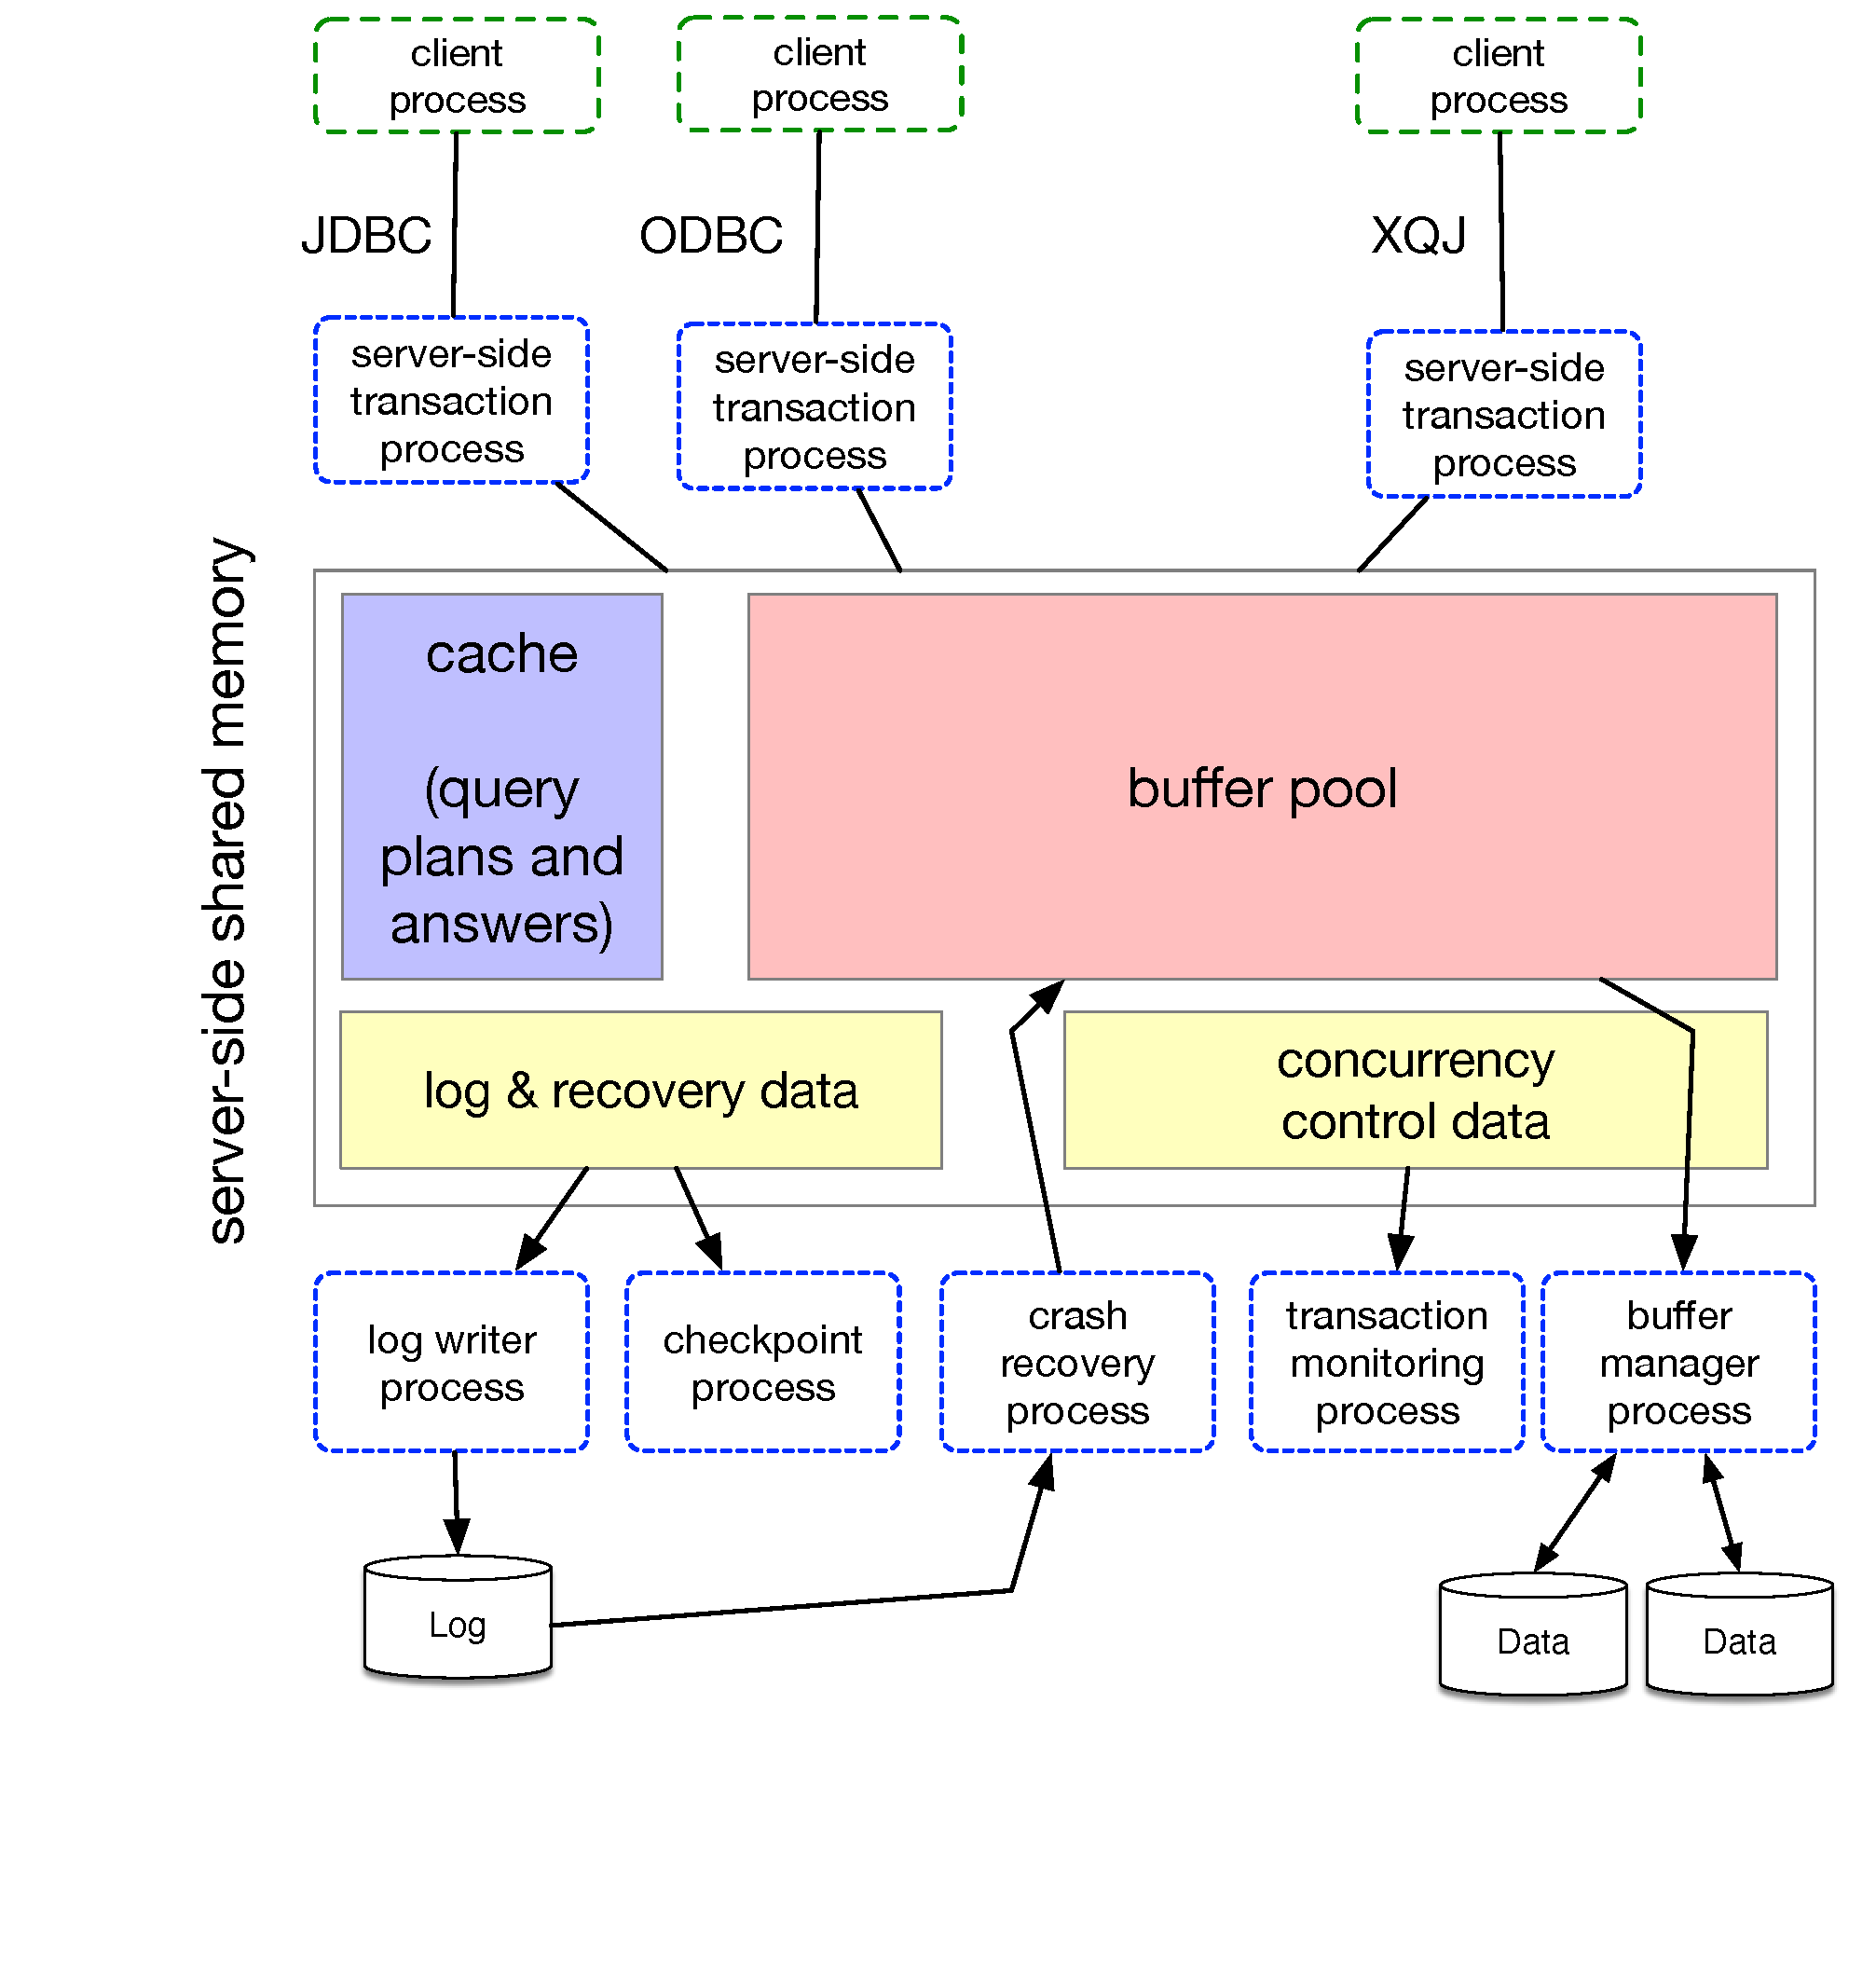
\includegraphics[width=1.1\textwidth]{figures/processes_memory_disks.eps}
\end{column}
\end{columns}
\end{frame}

\begin{frame}{Too much data?}

\begin{columns}[onlytextwidth]
\begin{column}{0.5\textwidth}
``Large'' databases nowadays are measured in \textbf{peta}bytes.

\vskip1em
Financial institutions and retailers are probably among the ones with the largest relational databases out there.
\end{column}
\begin{column}{0.4\textwidth}
\includegraphics[width=1.1\textwidth]{figures/multiples_of_bytes.png}
\end{column}
\end{columns}

Some known very large databases:
\begin{itemize}[-,noitemsep,topsep=-10pt]
\item Facebook reported having a 30PB database in 2011
\item Google Maps was reported as 20PB in 2012
\item Google's crawl and associated metadata is reported at 10 exabytes
\item Scientific databases are often astronomical (in size too)
\end{itemize}
\end{frame}

\begin{frame}

\vskip3em

\begin{columns}[onlytextwidth]
\begin{column}{0.35\textwidth}
\begin{minipage}{1.25\textwidth}
\raggedright

With a large database, even the simplest queries become a challenge.

\vskip0.5em

Not too long ago, Google stored 25 billion pages. 

\vskip0.5em

At 20KB per page (ignoring figures, etc.), that would be 500 TB of raw data.
\end{minipage}
\end{column}
\begin{column}{0.45\textwidth}
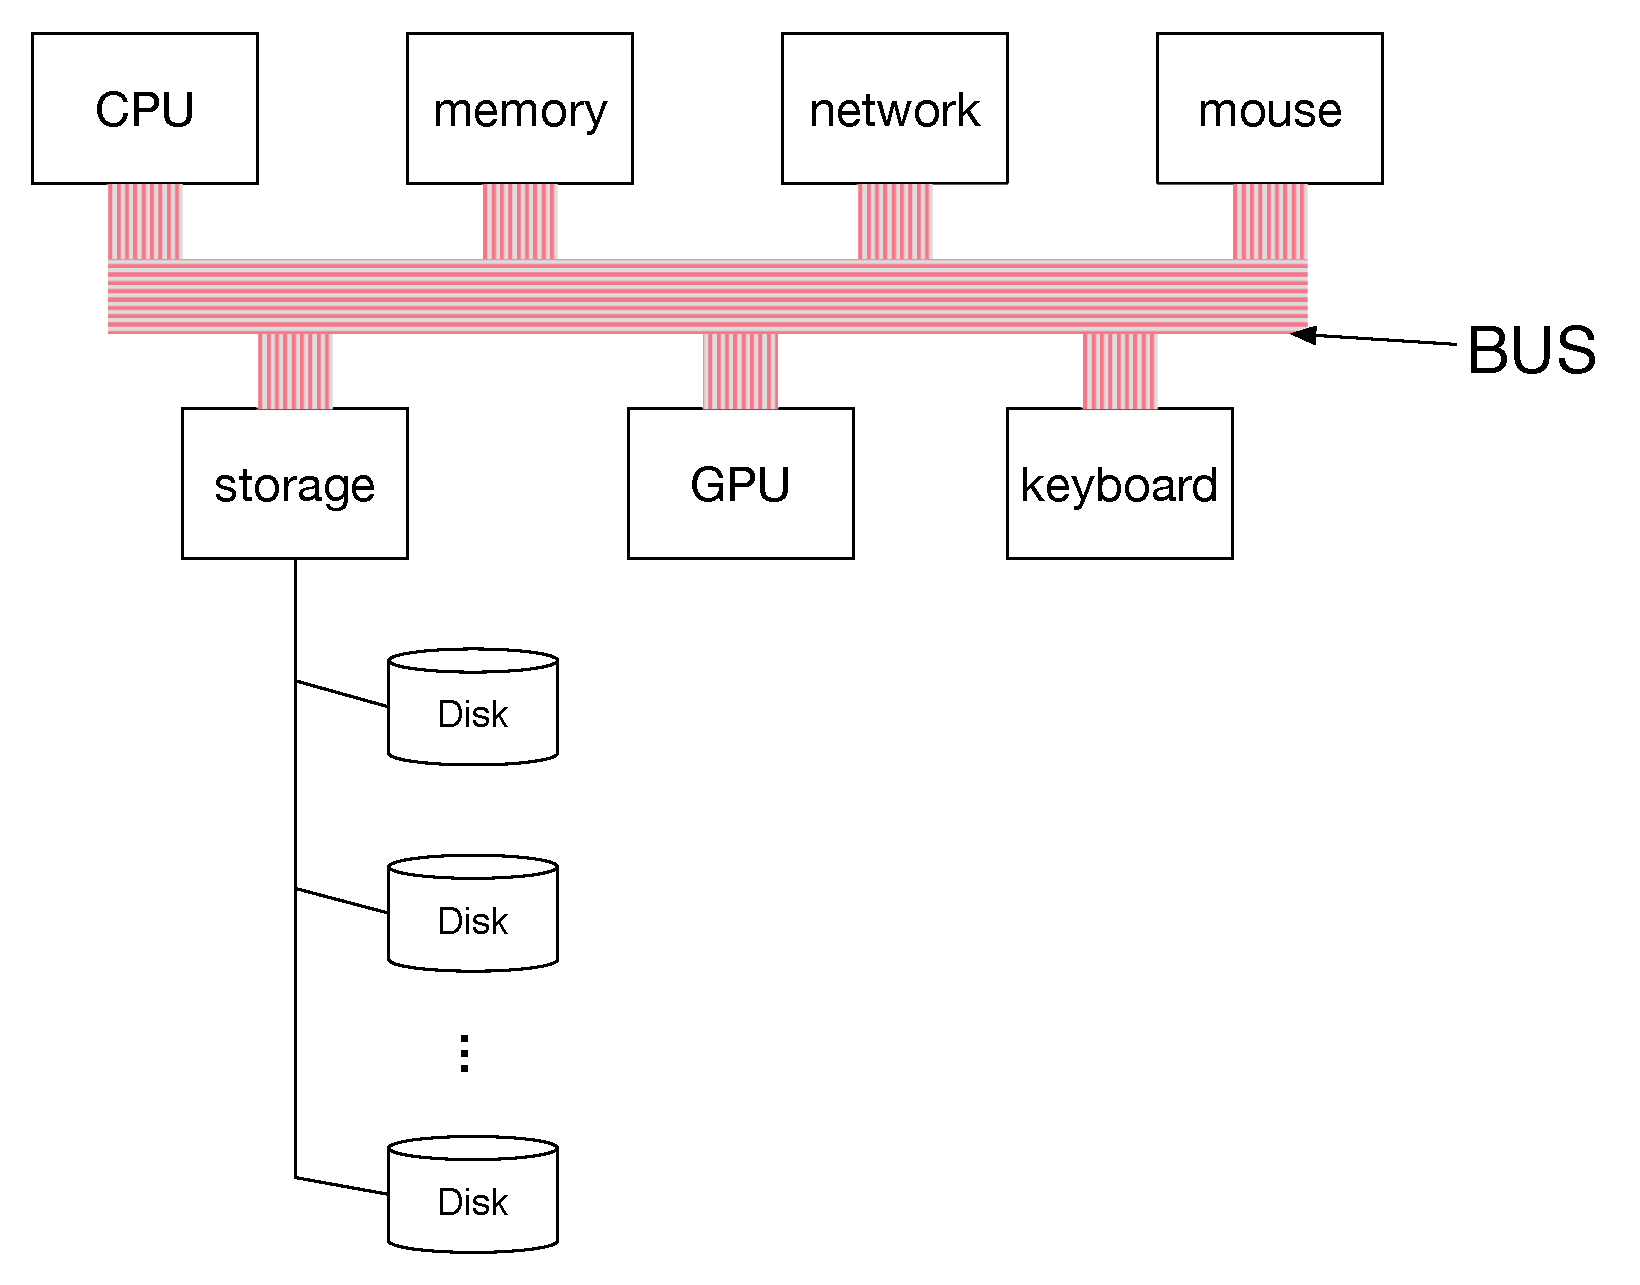
\includegraphics[width=1.1\textwidth]{../lec03_hardware/figures/von_neumann_architecture.eps}
\end{column}
\end{columns}

\vskip0.5em

How long would it take to run a query to find which web pages contain a link to \lstinline!ualberta.ca! on a ``standard server''?

With a fast 500MB/s BUS, \alert{the table scan would take at least}
\[\frac{500\cdot1024\cdot 1024 \text{ MB}}{500 \text{MB/s}}=1 M \text{seconds} \approx \text{ \alert{12 days}}\]
\end{frame}



\begin{frame}{Too many users?}

\begin{columns}[onlytextwidth]
\begin{column}{0.45\textwidth}
\begin{minipage}{1.25\textwidth}
\raggedright

Each connection to the database requires a ``server-side'' process which takes resources (memory for buffers).

\vskip0.5em

Also, each server-side process competes with the DBMS's own processes for CPU cycles.

\vskip0.5em

With a single CPU and 1,000 connected users, each requiring 1 second, it will take up to 15 minutes to serve them all.
\end{minipage}
\end{column}
\begin{column}{0.45\textwidth}
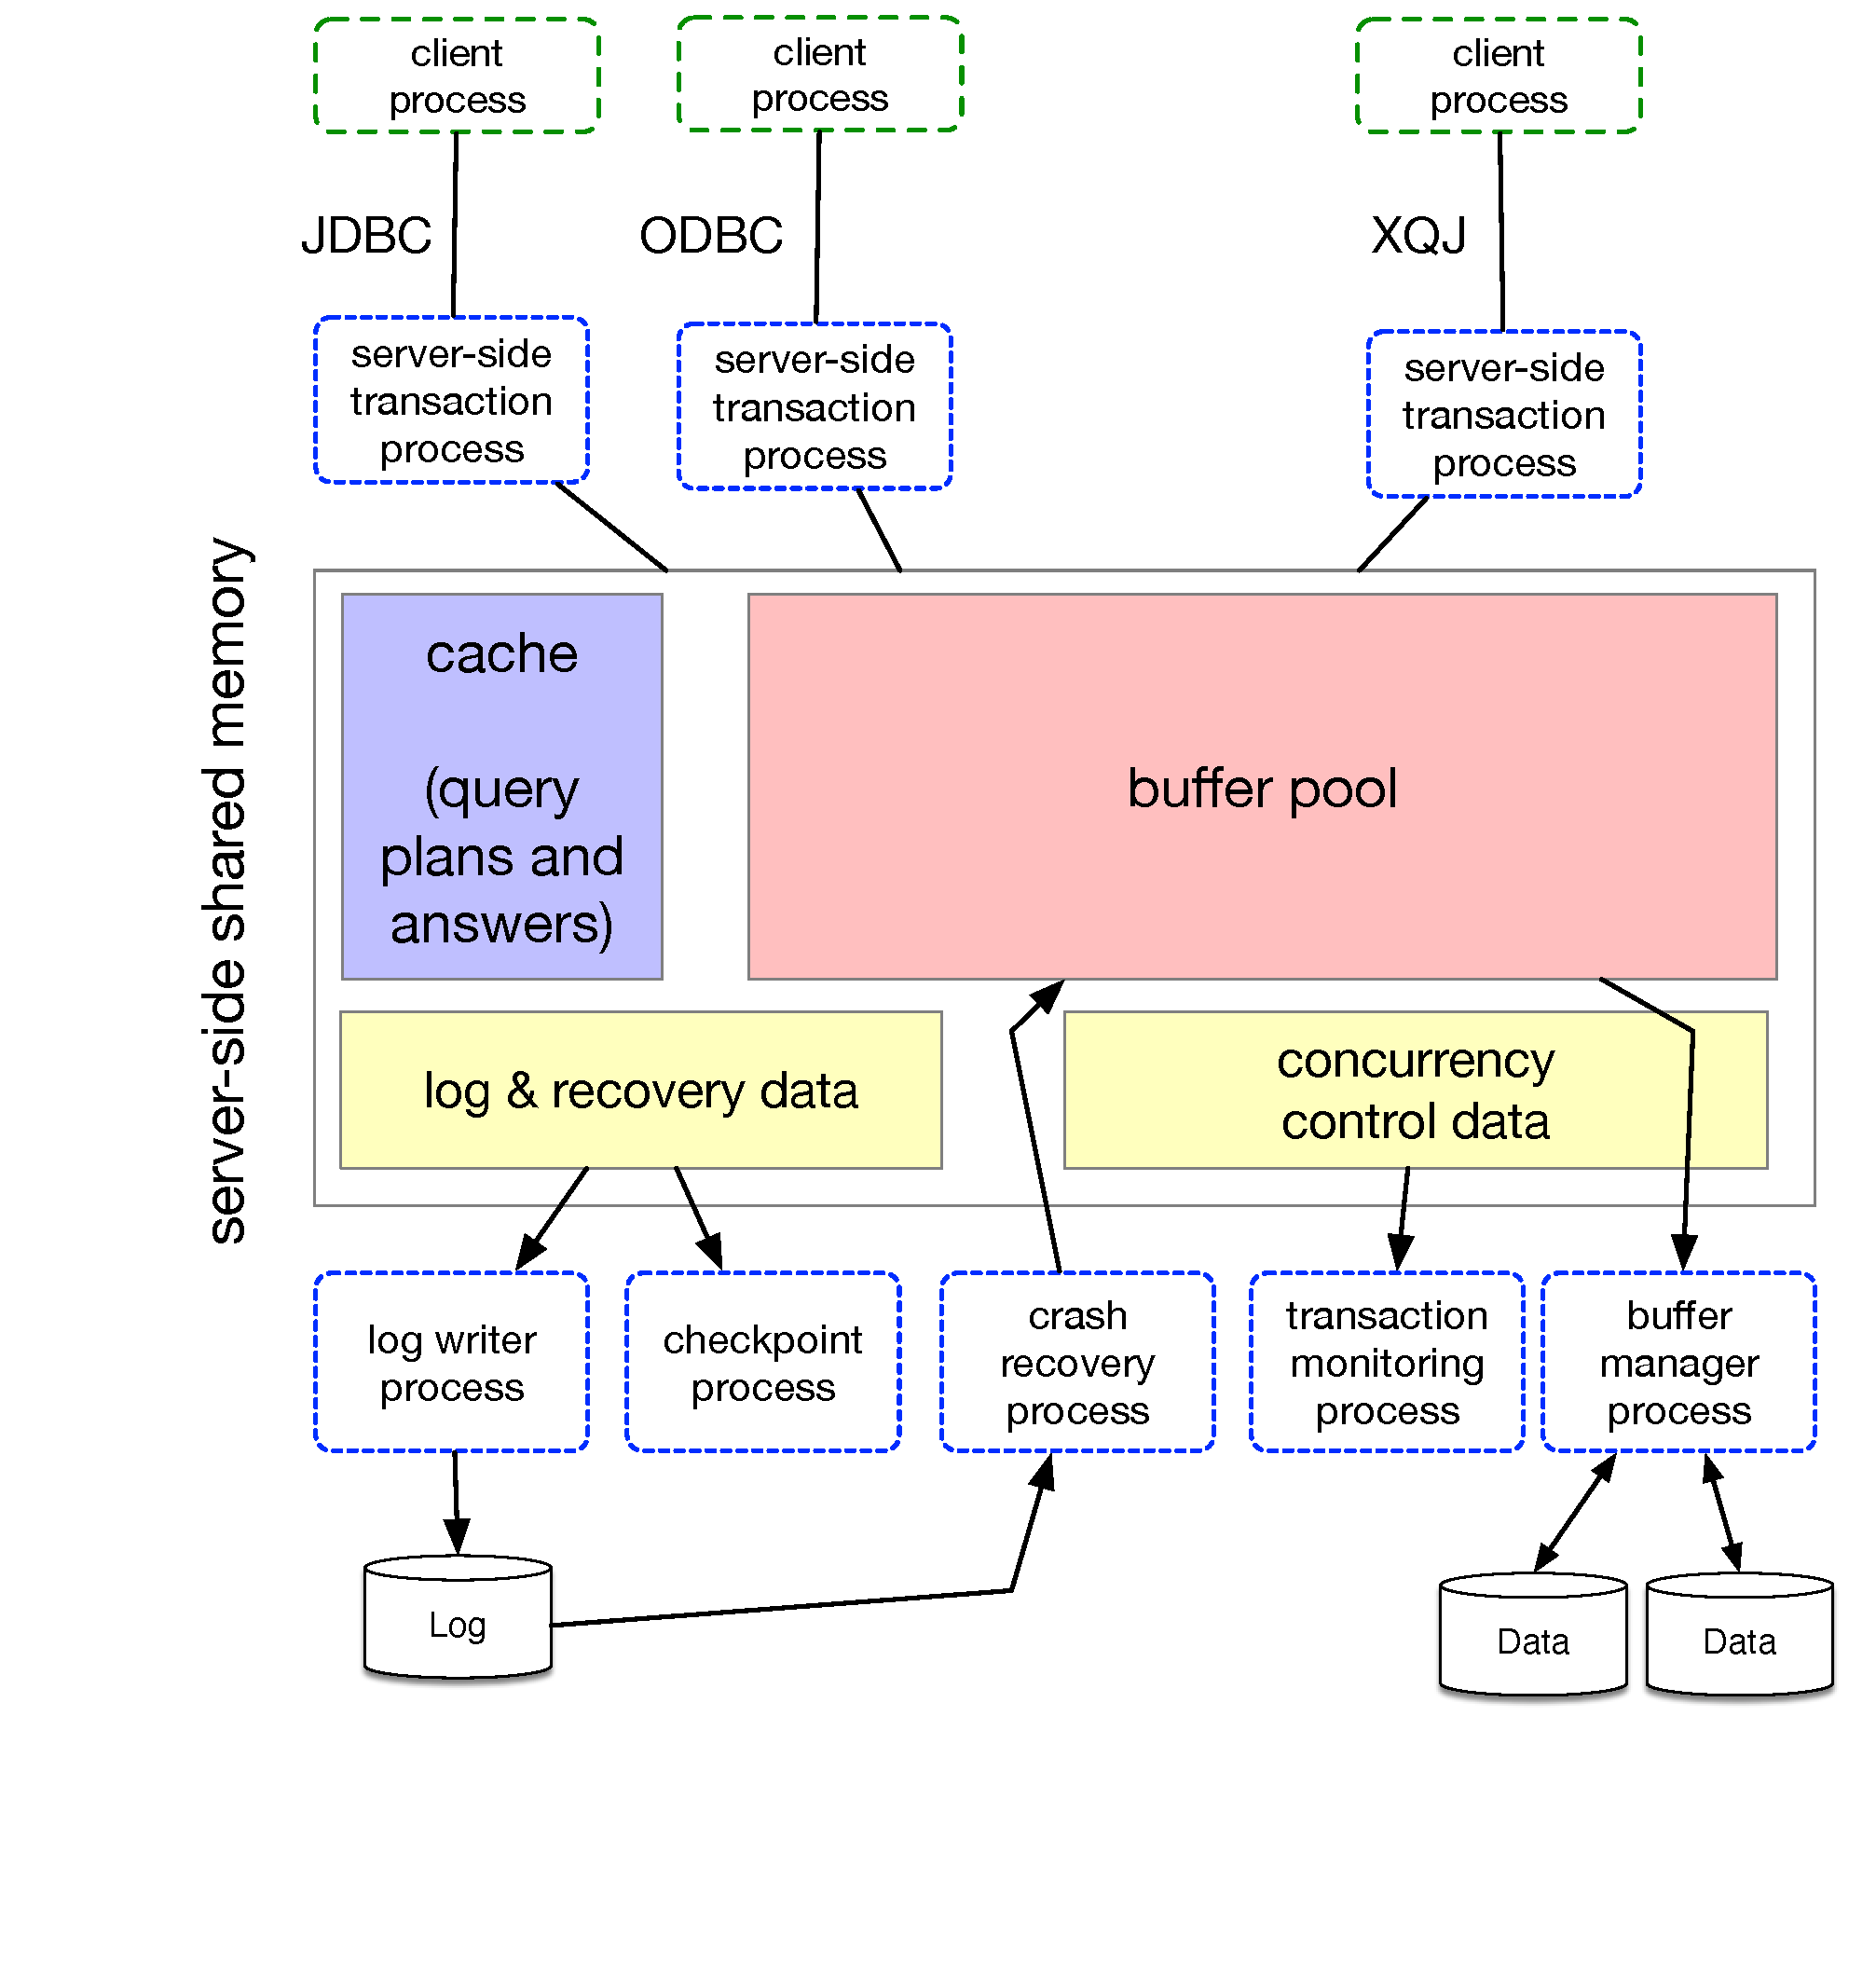
\includegraphics[width=1.1\textwidth]{figures/processes_memory_disks.eps}
\end{column}
\end{columns}
\end{frame}

\begin{frame}{Architectures for High Performance Computing}


\begin{columns}[onlytextwidth]
\begin{column}{0.45\textwidth}
The most modest step up from a standard Von Neumann architecture is to use a multi-core\footnotemark CPU:
\end{column}

\begin{column}{0.5\textwidth}
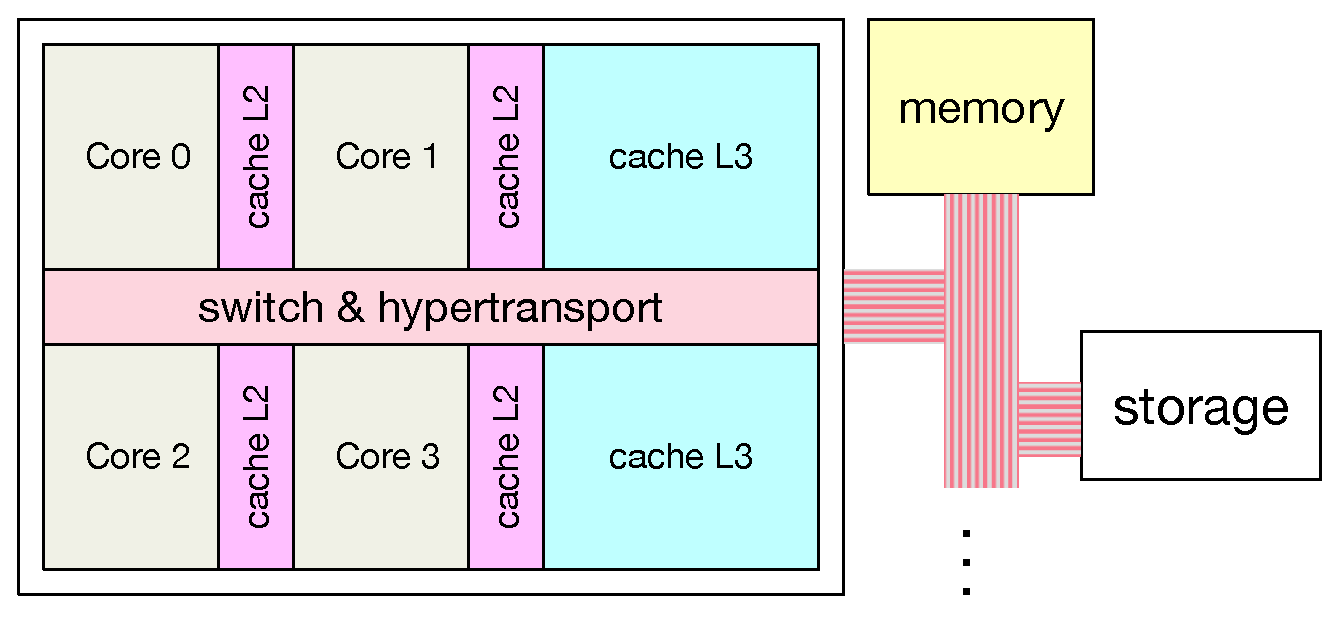
\includegraphics[width=1\textwidth]{figures/multicore.eps}
\end{column}
\end{columns}

Pros:
\begin{itemize}[-,noitemsep,topsep=-10pt]
\item \alert{Real parallelism}: as many DBMS processes as the number of cores running at the same time.
\item Can move a process from one core to another if needed.
\end{itemize}

\vskip1em

Cons:
\begin{itemize}[-,noitemsep,topsep=-10pt]
\item The BUS becomes a bottleneck!
\end{itemize}

\vskip1em

\footnotetext{\url{https://en.wikipedia.org/wiki/Multi-core_processor}}

\end{frame}


\begin{frame}

Modern ``single-box'' HPC servers have independent (multi-core) CPUs, each with its own memory, interconnected by a fast switch.

\vskip1em

\begin{center}
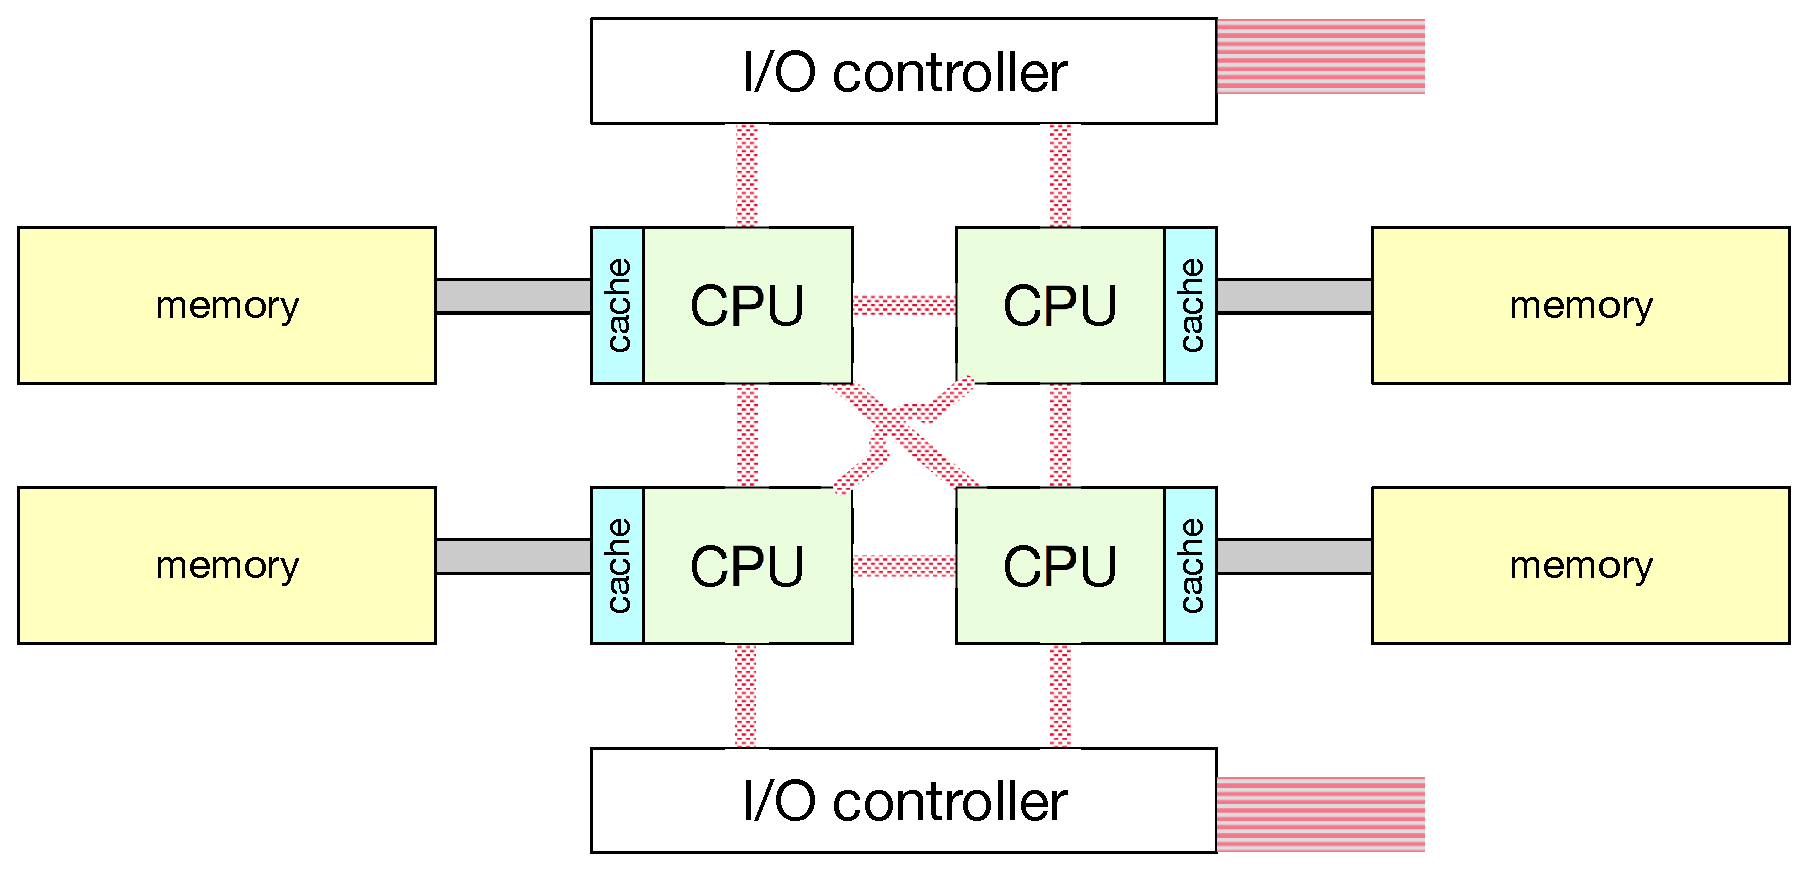
\includegraphics[width=0.75\textwidth]{figures/numa_architecture.eps}
\end{center}

\vskip1em

Processes on different CPUs can \alert{share memory}, but with a Non-Uniform Memory Access (\textbf{NUMA}\footnote{\url{https://en.wikipedia.org/wiki/Non-uniform_memory_access}}) cost: accessing local memory is cheaper.
\end{frame}


\begin{frame}{Shared Data Architectures}

When NUMA is not enough, we \alert{move \textbf{up}} to clusters of computers that shared only the data on disk:

\begin{center}
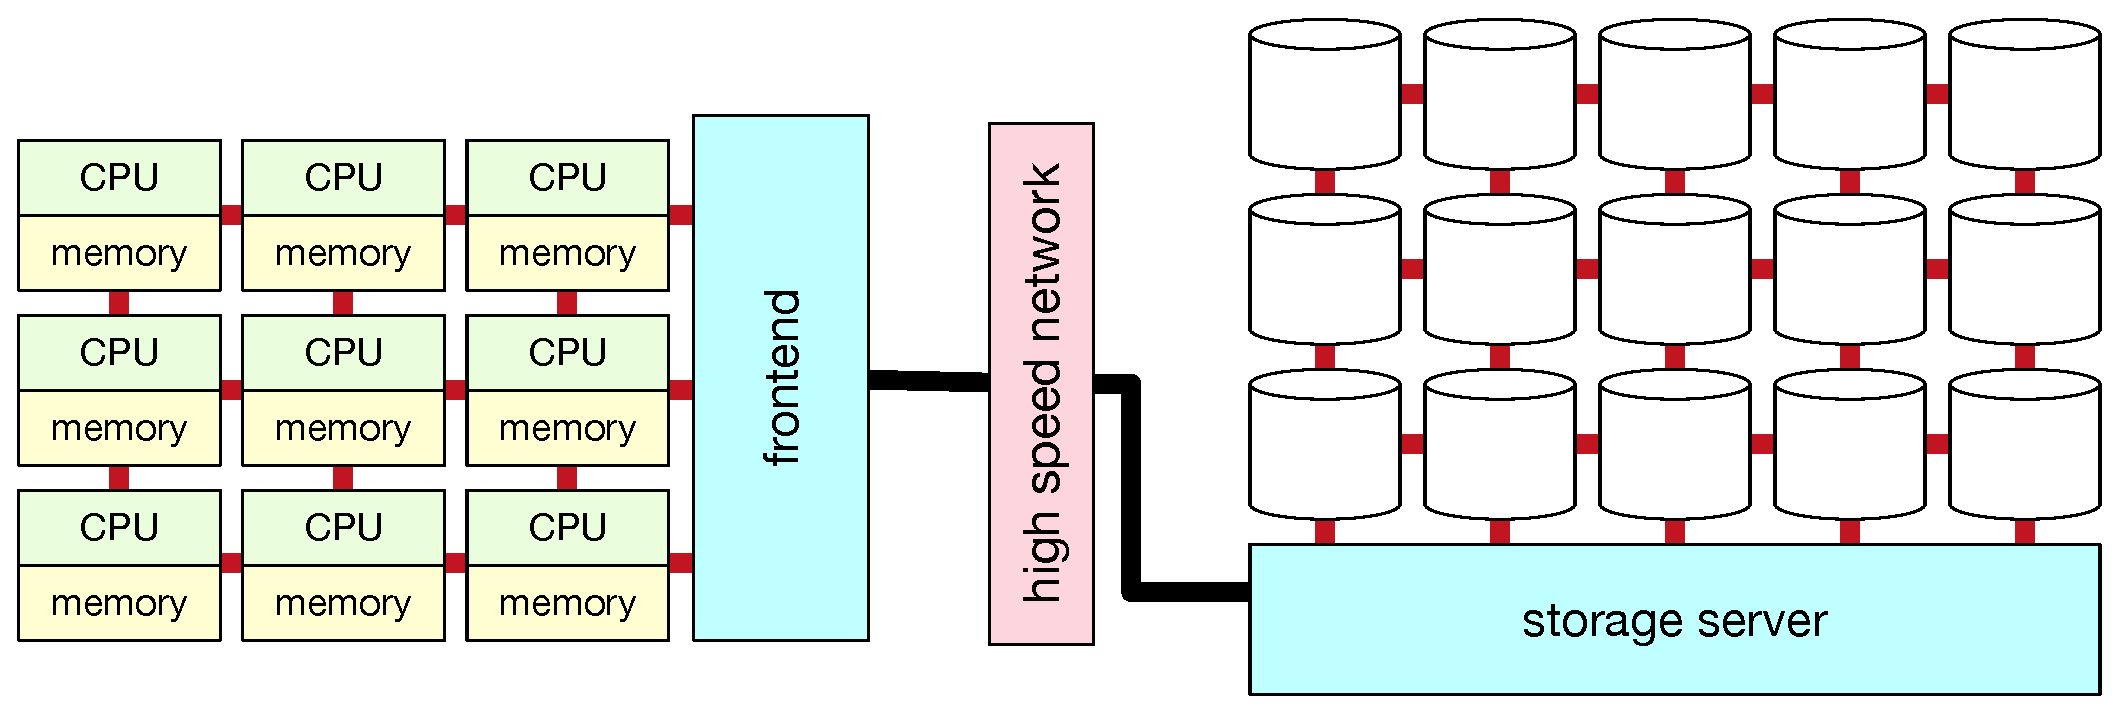
\includegraphics[width=0.75\textwidth]{figures/shared_disk_SAN.eps}
\end{center}

``Single-node DBMS'' in this architecture: transaction processes and DBMSs process run on separate nodes and communicate via a local network.

However, transferring data from the storage array becomes a bottleneck. A fast network can reach up to 5GB/s, but that would still mean 1 day to transfer 500 TB each way.

\end{frame}

\begin{frame}{Shared Nothing Architectures}

\begin{center}
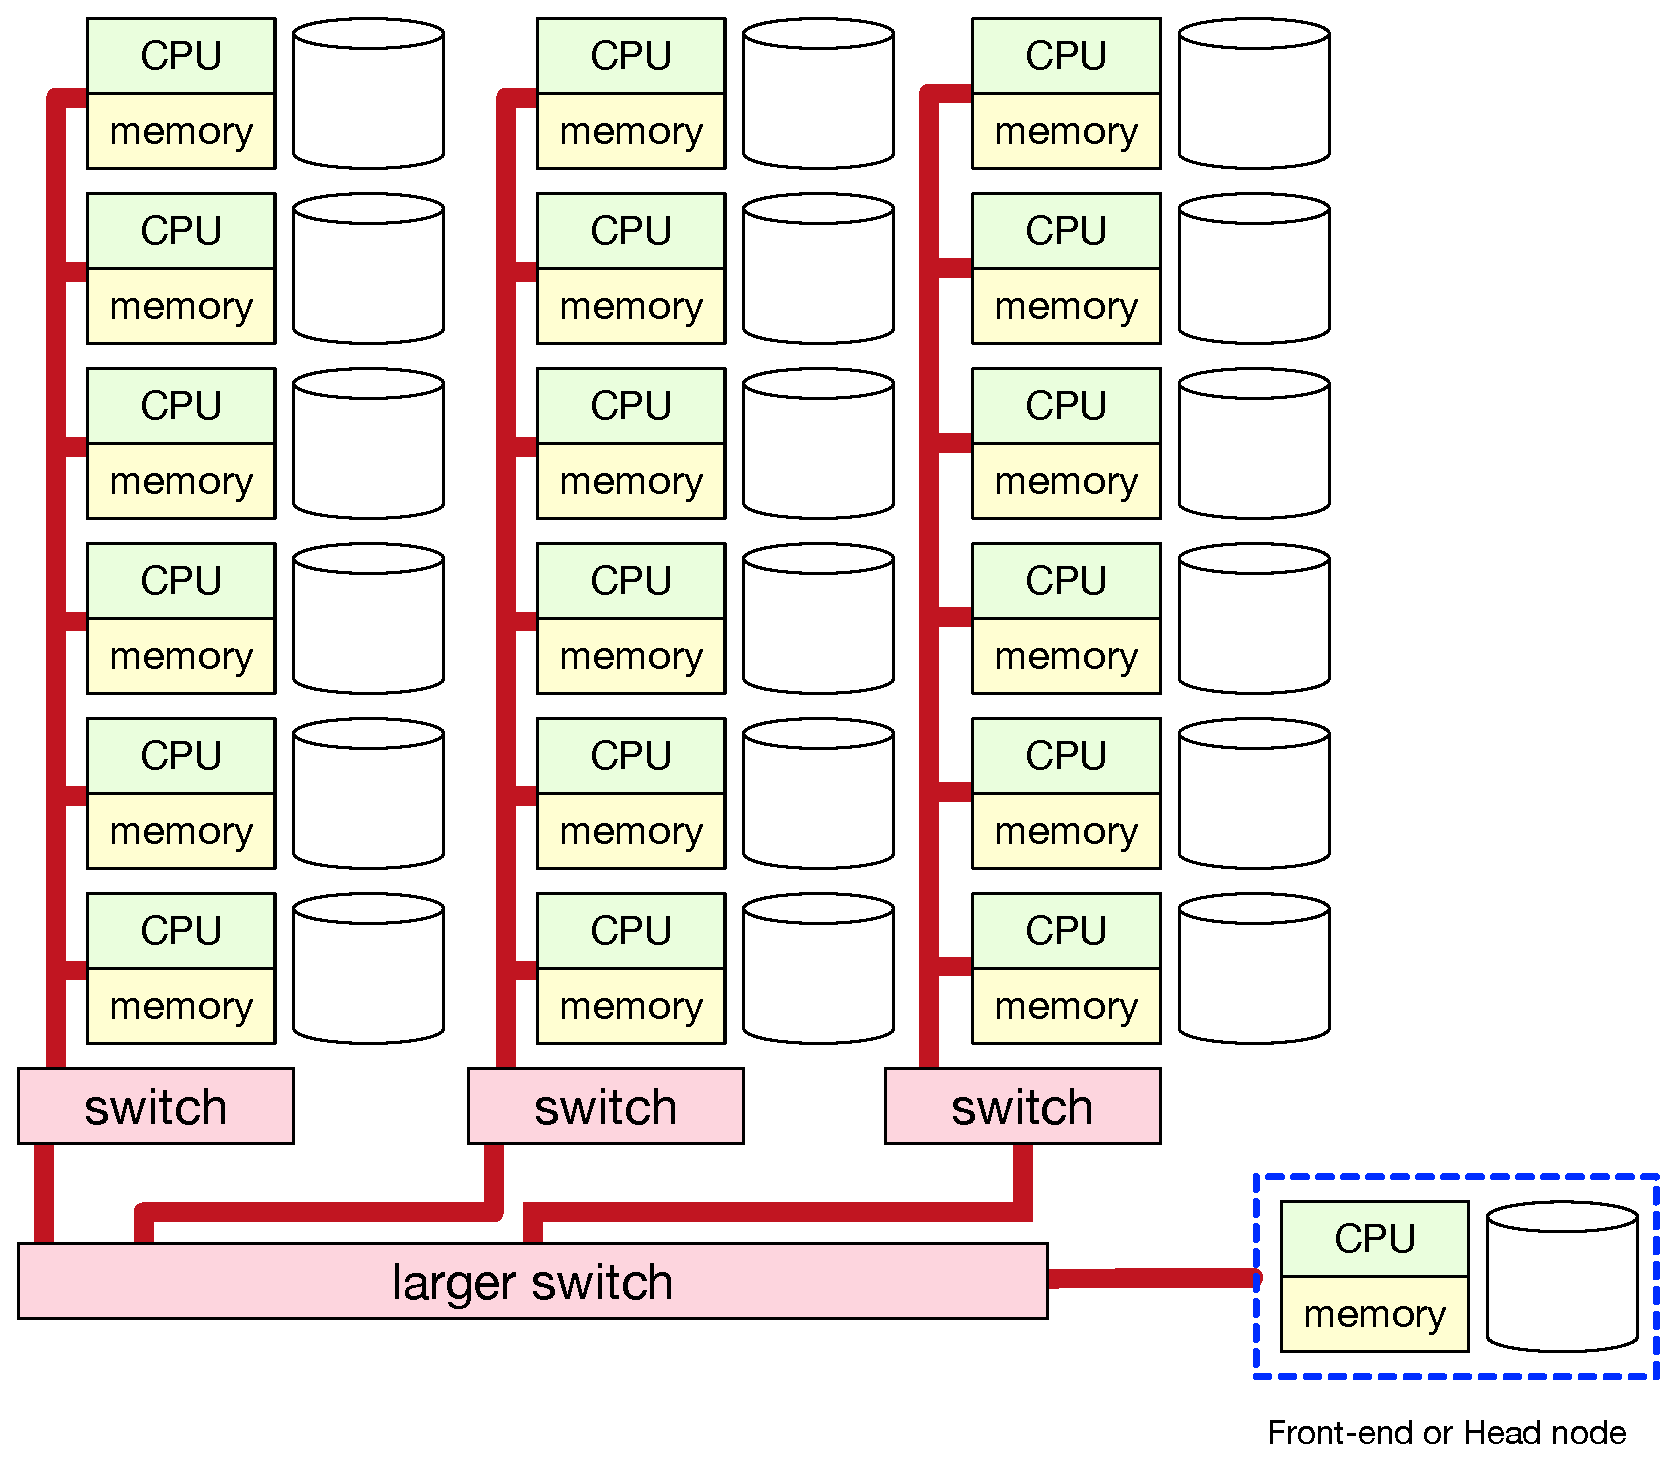
\includegraphics[width=0.75\textwidth]{figures/shared_nothing.eps}
\end{center}
\end{frame}

\begin{frame}{Why is Shared Nothing so Popular?}

Shared nothing architectures are made up of \alert{inexpensive} computing nodes, each with its own disk and memory (typically about \$1000 per node).

Shared nothing is ideal for \alert{scaling \textbf{out}} (instead of up): if you need more computing power, buy a few more computing nodes and hook them to the existing cluster.

\vskip1em

Shared nothing is great for \textbf{\alert{embarrassingly parallel}} workloads: spread the data among the nodes and run the same query (e.g., finding pages with links to \lstinline!ualberta.ca!) on every node at the same time.

\end{frame}

\begin{frame}{Virtualization and cloud computing}

Computing clouds are clusters of (shared-nothing) nodes that host a large number of virtual machines (VMs), each with their own OS.
\begin{itemize}[-]
\item Multiple VMs run simultaneously on the same physical node.
\item VMs can migrate across nodes (like processes migrate across processors).
\end{itemize}

\vskip1em


\end{frame}

\begin{frame}{Cloud Computing can Save (a lot!)}

Running an enterprise-scale datacenter incurs many costs:
\begin{itemize}[-,noitemsep]
\item Infrastructure: building maintenance, electricity, cooling, ...
\item Expertise: good IT staff costs a lot!
\end{itemize}

If the organization \textbf{under}-provisions (i.e., the IT infrastructure is too small), then it loses customers until it grows.

If the organization \textbf{over}-provisions (i.e., the IT infrastructure is too big), then it wastes money in maintenance cost.

\vskip1em

\begin{block}{Clouds $\approx$ Outsourced Infrastructure}
\alert{Main advantage}: let experts run the IT infrastructure and pay only for what you need (or what you use).
\end{block}
\end{frame}

\begin{frame}{Clouds continued}

\alert{Infrastructure as a Service} (IaaS):
\begin{itemize}[-,noitemsep,topsep=-10pt]
\item The cloud hosts ``bare bones'' VMs and the user installs their own OS and software stack
\end{itemize}

\alert{Platform as a Service}:
\begin{itemize}[-,noitemsep,topsep=-10pt]
\item The cloud offers self-managing VMs that implement a specific service
\begin{itemize}[-,noitemsep,topsep=-5pt]
\item email, word processing, other office applications
\item database services: MySQL, PostgreSQL, ...
\item document storage: MongoDB, CouchDB, ...
\item key/value ``data stores'': Bigtable, Cassandra, HBase, ...
\end{itemize}
\end{itemize}

\vskip1em

Google: {\footnotesize\url{https://cloud.google.com/products/\#databases}}

Amazon: {\footnotesize\url{https://aws.amazon.com/products/databases/}}
\end{frame}

\begin{frame}{Clouds bring economies of scale}

\begin{columns}[onlytextwidth]
\begin{column}{0.5\textwidth}
\begin{block}{\alert{Elasticity}}
Increasing/decreasing the number of VMs providing any service in response to changes in demand.
\end{block}

\begin{block}{Scaling \alert{Out}}
Growth by adding new physical nodes to cope with demand.
\end{block}
\end{column}
\qquad
\begin{column}{0.5\textwidth}
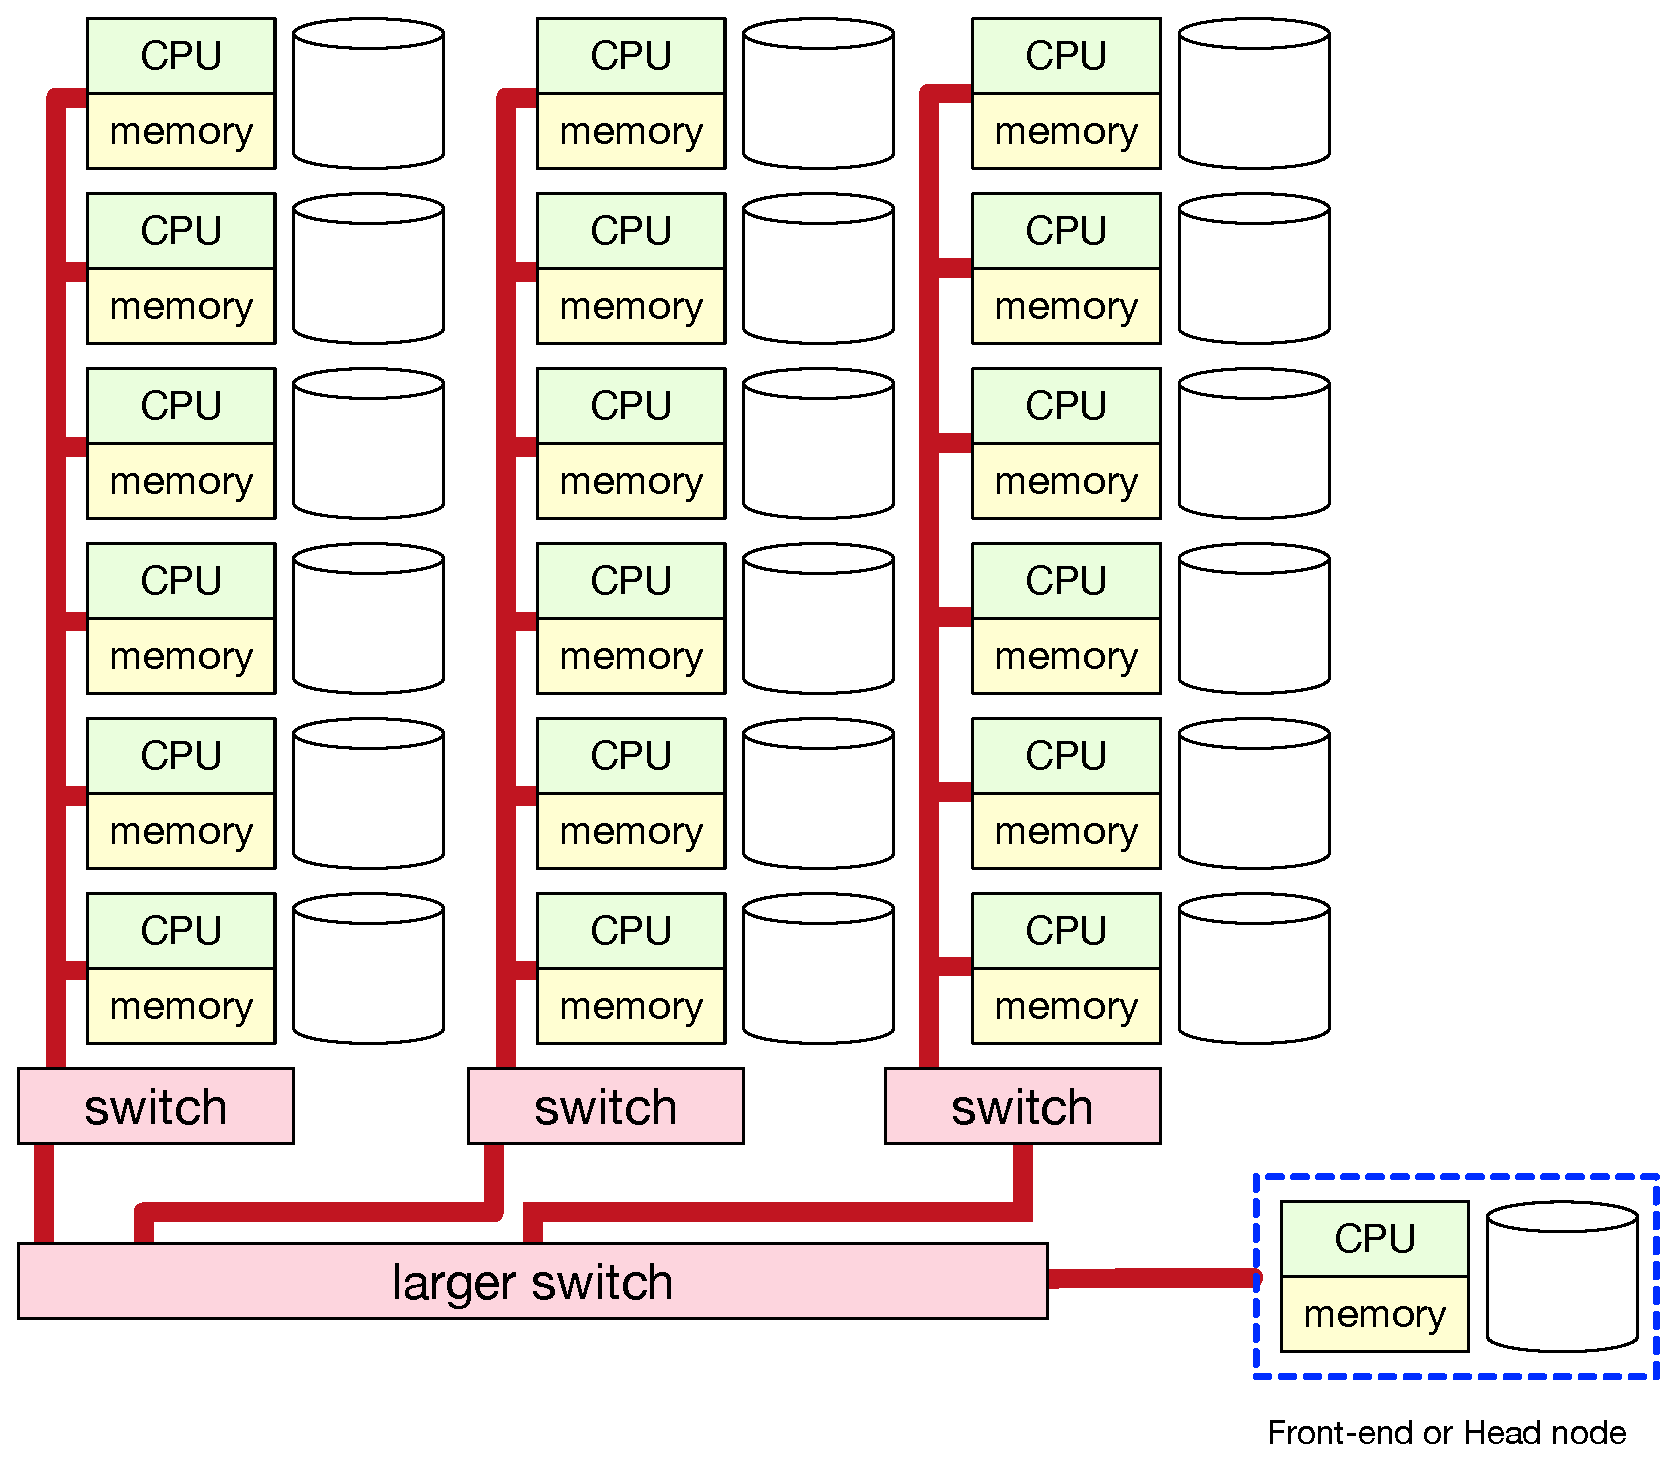
\includegraphics[width=0.9\textwidth]{figures/shared_nothing.eps}
\end{column}
\end{columns}

\vskip1em

\begin{block}{\alert{Multi-tenancy}}
Different clients have their VMs (or database services) running simultaneously on the same physical cluster.
\end{block}
\end{frame}


\begin{frame}{Redundancy is essential}
\begin{itemize}[-]
\item The cluster components (compute nodes and network connections) are inexpensive and will break at some point
\begin{itemize}[-,noitemsep]
\item Most clusters use commodity hardware; 
\item Google, Amazon and other massive IT companies have started to design their own custom compute nodes 
\end{itemize}
\item A data center with thousands of nodes will experience several node failures every day
\item \alert{Challenge \#1}: restarting the computation after each failure is not an option.... the computation model has to be \alert{\textbf{fault tolerant}}
\end{itemize}

\begin{block}{}
\alert{Redundancy} is one way of being fault tolerant: store the same on different compute nodes, across different cluster racks.
\end{block}
\end{frame}


\begin{frame}{Speedup and Scaleup}

\vskip1em

\begin{columns}[onlytextwidth]
\begin{column}{0.5\textwidth}
\centering
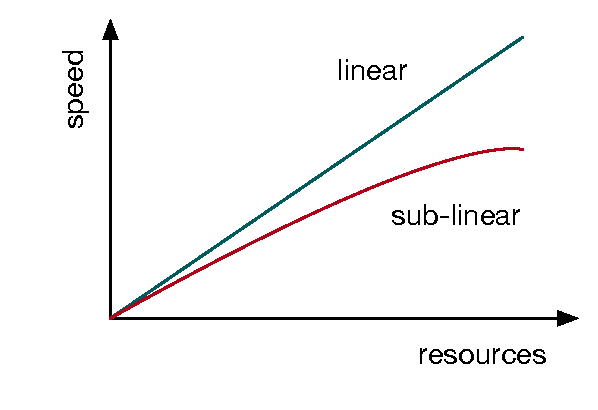
\includegraphics[width=\textwidth]{figures/speedup.eps}

Speedup
\end{column}
\begin{column}{0.5\textwidth}
\centering
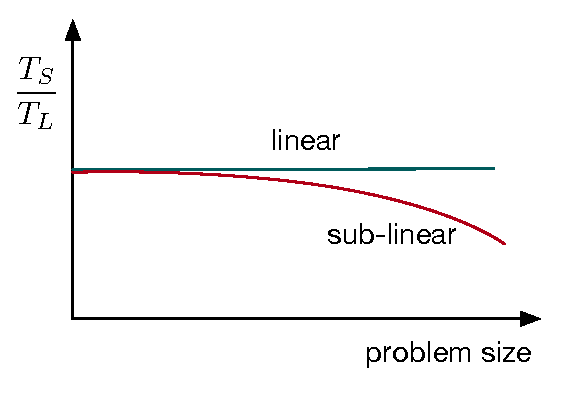
\includegraphics[width=\textwidth]{figures/scaleup.eps}

Scaleup
\end{column}
\end{columns}

\alert{\textbf{Speedup}} measures how much faster the system accomplishes a task as more computing resources are added.

\alert{\textbf{Scaleup}} takes into account the growth of the database. $T_S$ is the time it takes to complete the task on the ``small'' computer, while $T_L$ is the time on the ``large'' computer.

\end{frame}

\begin{frame}{HPC trade-offs}

A \alert{perfect high performance computer} (parallel or distributed) would have \textbf{linear speedup and scaleup}.

In practice this does not happen. The more components in a system, the more time is needed for them to coordinate amongst themselves.

\begin{block}{Example}
\begin{itemize}[-,noitemsep]
\item A DBMS log writer process responds faster to a server-side transaction process running on the same CUP instead of a process running on a different CPU or a different computer.
\end{itemize}
\end{block}

\textbf{Synchronizing independent processes takes time} proportional to the complexity of the computer. Also, we have to account for failures and build redundant checks (which also take time).
\end{frame}


\begin{frame}{Synchronization in DBMS workloads}

\textbf{Fact}: synchronization time grows with system complexity.

\alert{\textbf{Corollary}}: tasks that do not require synchronization show better speedup and scaleup.

\vskip1em


\begin{block}{\alert{\textbf{ACID transactions}} require a lot of synchronization}
\begin{itemize}[-,noitemsep,topsep=-10pt]
\item Atomicity requires logging.
\item Isolation requires transaction monitoring, locking, etc. which \underline{must be performed} by a single DBMS process.
\end{itemize}
\end{block}

A defining ``feature'' of many NoSQL systems that scale well is to not provide ACID transactions.

\end{frame}



\begin{frame}{Parallel vs Distributed Database}

In a single-node parallel database all the data and all DBMS processes reside in the same HPC computer, independently of architecture:

\vskip1em

\begin{columns}[onlytextwidth]
\begin{column}{0.3\textwidth}
\centering 
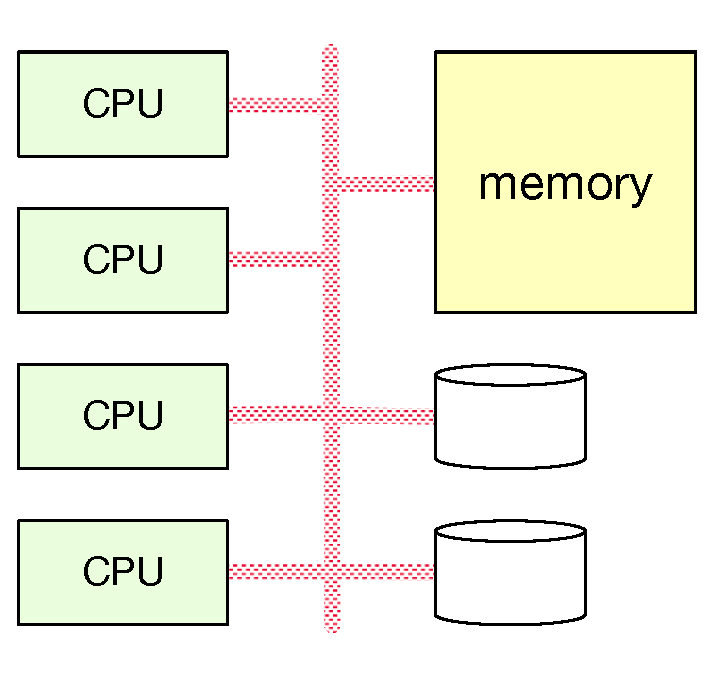
\includegraphics[width=0.75\textwidth]{figures/shared_memory_simplified.eps}

\footnotesize shared memory
\end{column}

\qquad \begin{column}{0.3\textwidth}
\centering 
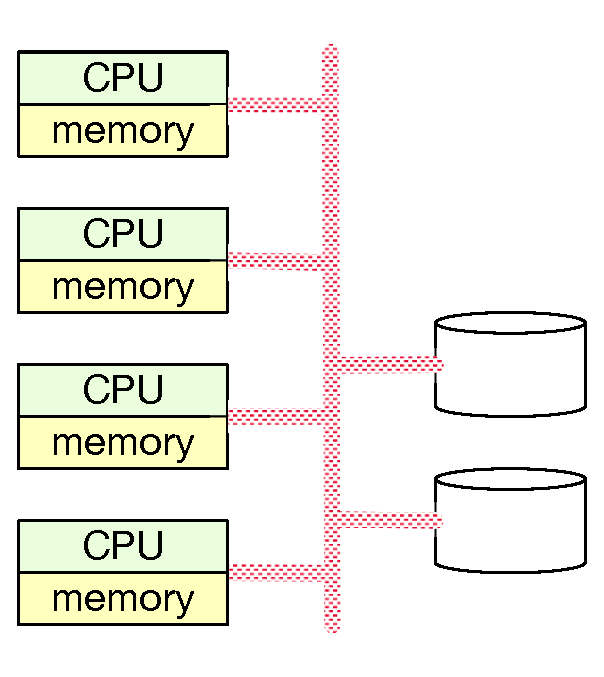
\includegraphics[width=0.75\textwidth]{figures/shared_disk_simplified.eps}

\footnotesize shared disk
\end{column}

\qquad \begin{column}{0.3\textwidth}
\centering 
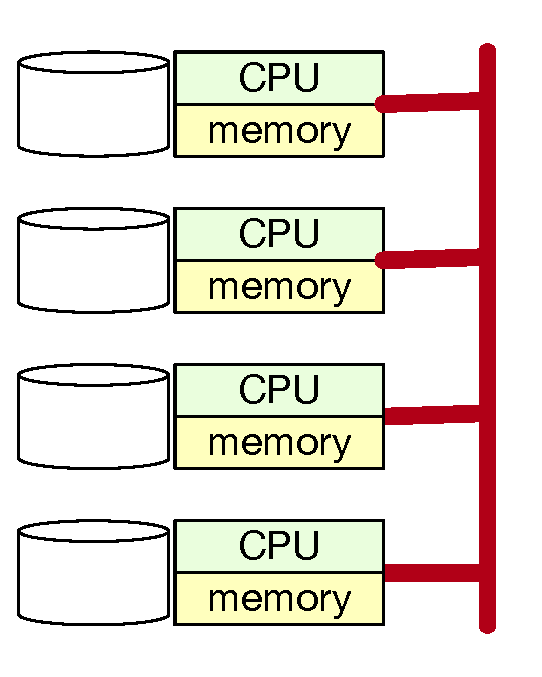
\includegraphics[width=0.75\textwidth]{figures/shared_nothing_simplified.eps}

\footnotesize shared nothing
\end{column}
\end{columns}

\vskip1em

A distributed database is one made of autonomous ``single-node'' databases. Typically, each database is located on a different data center (i.e., the nodes are geographically dispersed).

\end{frame}

\begin{frame}

We fill focus on shared-nothing clusters, as they are becoming the most popular (due to the cost benefits of cloud computing).

\vskip1em

Main questions about HPC NoSQL in the remaining of the notes:
\begin{itemize}[-]
\item What data management problems are shared nothing architectures best for?

\item What compromises do we make to handle more data or clients relative to what a single-node relational system offers?
\end{itemize}
\end{frame}